%!TEX root = main.tex



\section{Results}


\begin{frame}
\frametitle{$M_{jj}$ and $p_\mathrm{T,pair}$ - pp v.s p-Pb }

\begin{columns}[t]
\column{.5\textwidth}
\centering
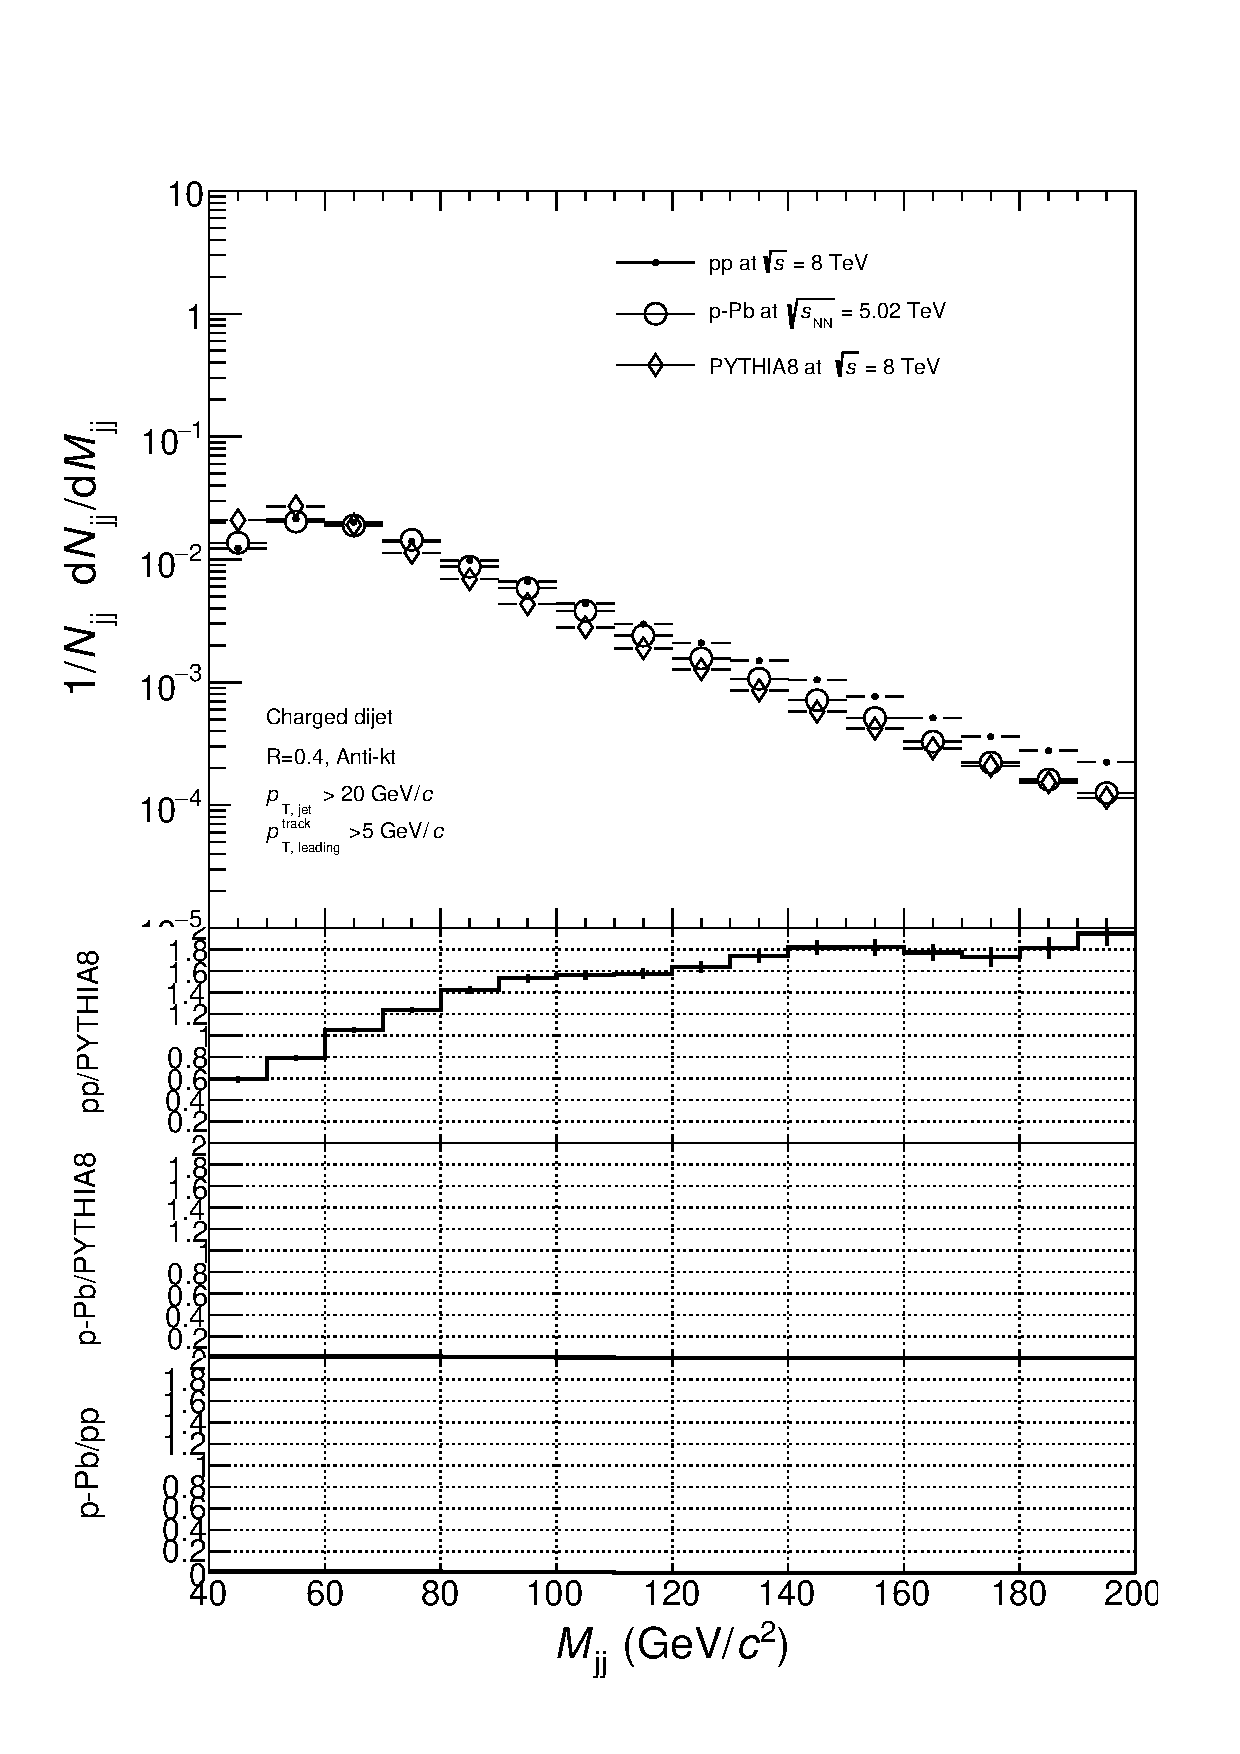
\includegraphics[width=1\linewidth]{mjj_13d_pp_pPb}\\
\column{.5\textwidth}
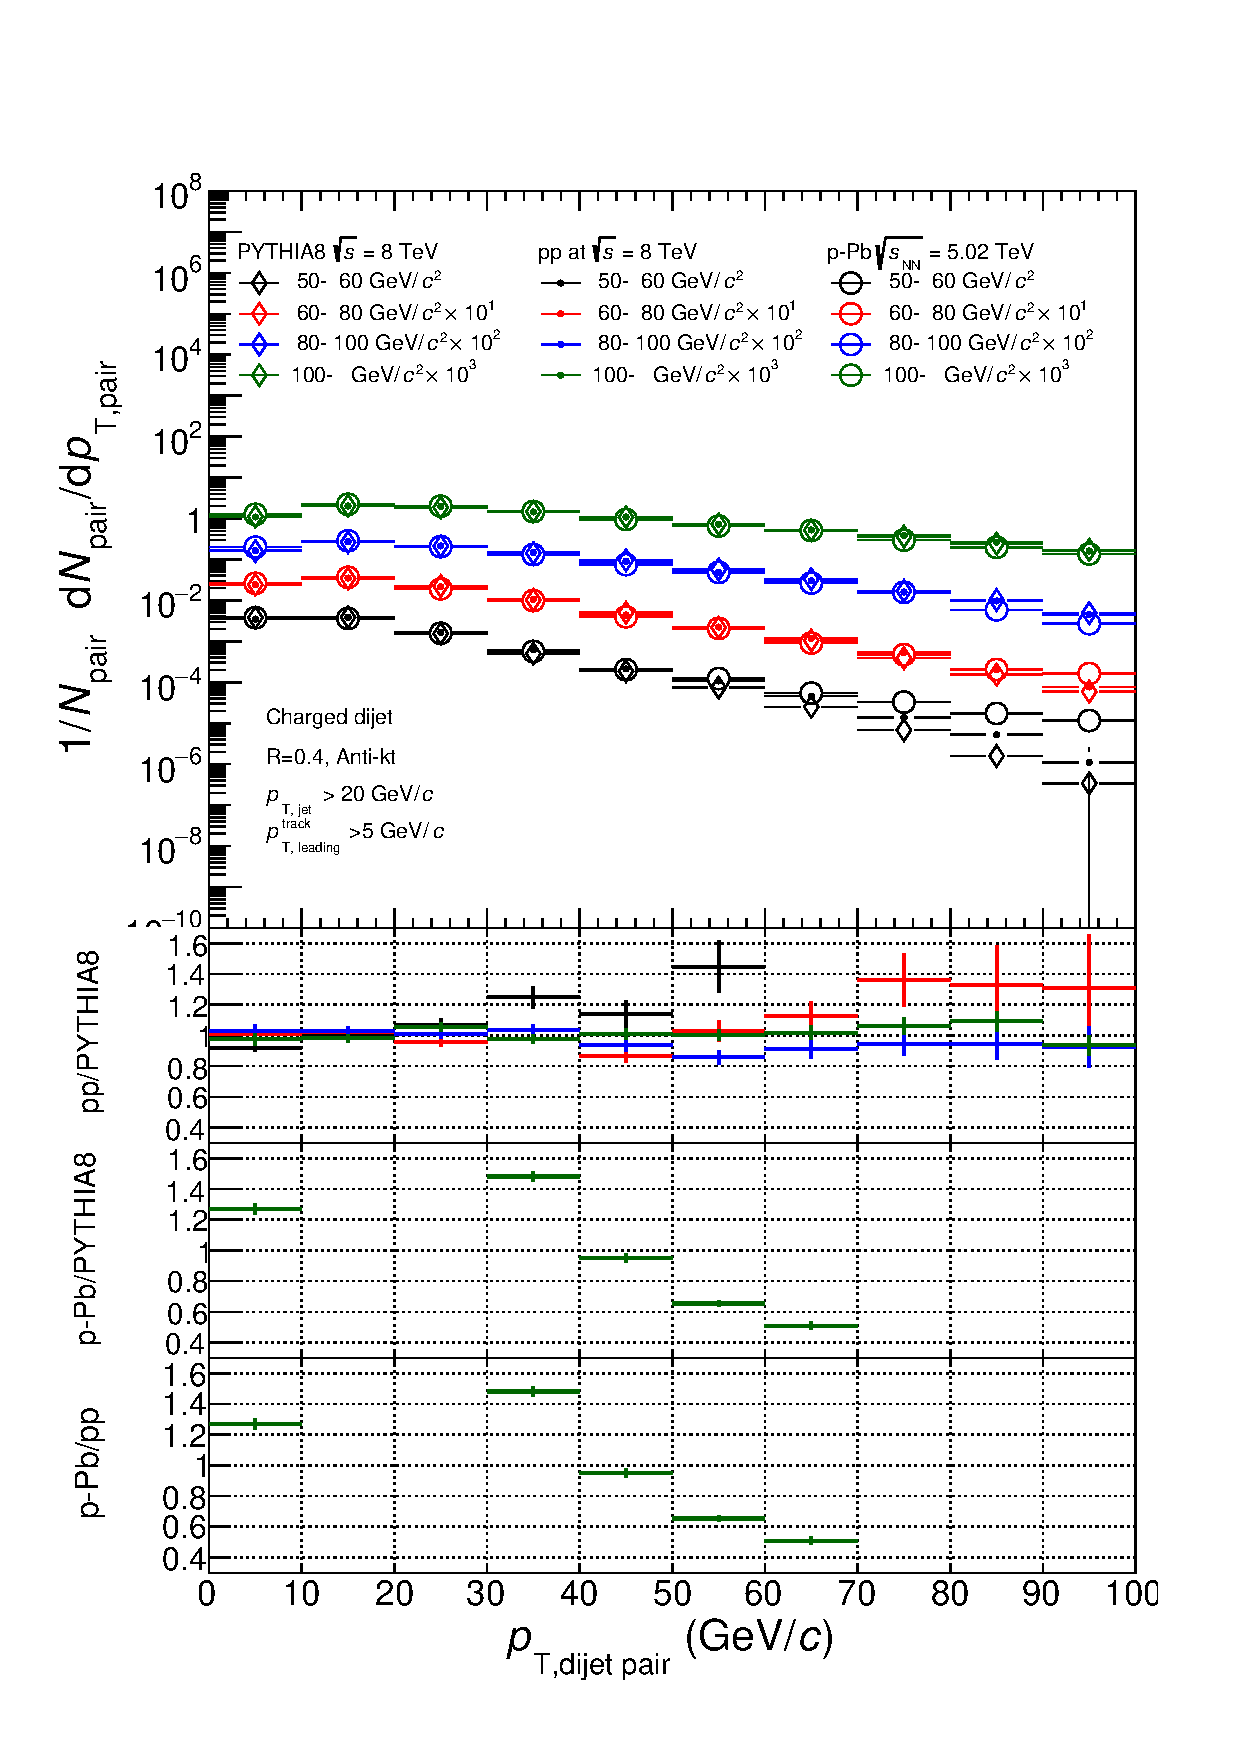
\includegraphics[width=1\linewidth]{ptjj_13d_pp_pPb}\\
\end{columns}
\end{frame}
%begin{frame}
%\frametitle{Systematic uncertainty}
%Take into account sources below 
%\begin{itemize}
%	\item{$p_\mathrm{T}$ smearing due to the underlying event}
%	\item{Tracking efficiency of charged tracks}
%	\item{Unfolding process for the both $M_\mathrm{dijet}$ and $p_\mathrm{T.pair}$}
%\end{itemize}

%\end{frame}


\begin{frame}
\frametitle{Summary}
$M_{jj}$ and $p_\mathrm{T,pair}$  of charged dijets 
\begin{itemize}
	\item for pp at $\sqrt{s} = 8$ TeV and p-Pb and Pb-p at $\sqrt{s_\mathrm{NN}}$ = 5.02 TeV 
	\item compared with PYTHIA6-2011 (for pp data) and PYTHIA8 (for p-Pb and Pb-p data)
	\item No cold-nuclear matter effect is shown in p-Pb collisions
	\item still ongoing for Pb-Pb data (flow background subtraction) to conclude the nuclear matter modification in the hot and dense medium
	\item finalizing the subjects for pp and p-Pb data
	\item Planning two papers ($M_{jj}$ and  $p_\mathrm{T,pair}$ separately) 
	\item extending the study with full jets
\end{itemize}

\end{frame}






